\documentclass[11pt,draftnofoot,onecolumn]{IEEEtran}

\def\spacingset#1{\def\baselinestretch{#1}\small\normalsize}

%\def\ninept{\def\baselinestretch{.95}\let\normalsize\small\normalsize}

\setlength{\topmargin}{-0.4in}             % Move the top margin up with the negative value.
\setlength{\textheight}{9.0in}                % Set the hight of the text.
\setlength{\textwidth}{6.9in}               % Set the width of the text.
\setlength{\oddsidemargin}{-0.2in}           % Set the odd side left margin; useful for the double-sided case.
\setlength{\evensidemargin}{-0.2in}

%\parskip=1pt
\usepackage{amssymb}
\usepackage{amsmath}
\usepackage{latexsym}
\usepackage{epsf}
%\usepackage{psfig}
\usepackage{graphicx}
%\usepackage{showkeys}
%------------------------------------------------------------------
%common definition file for Latex
%------------------------------------------------------------------

\def\bg{\Large}

%------------------------------------------------------------------
% Command for spacing:---------------------------------------------
\def\spacingset#1{\def\baselinestretch{#1}\small\normalsize}
\newcommand{\vs}{\vspace}
\newcommand{\hs}{\hspace}

%------------------------------------------------------------------
% Notations used in linear circuits and electronic devices:--------
\newcommand{\volt}{\, \mbox{V}}
\newcommand{\amp}{\, \mbox{A}}
\newcommand{\mamp}{\, \mbox{mA}}
\newcommand{\ohm}{\, \Omega}
\newcommand{\kohm}{\, \mbox{k}\Omega}
\newcommand{\watt}{\, \mbox{W}}
\newcommand{\kwatt}{\, \mbox{kW}}
\newcommand{\farad}{\, \mbox{F}}
\newcommand{\ufarad}{\, \mu\mbox{F}}
\newcommand{\henry}{\, \mbox{H}}
\newcommand{\mhenry}{\, \mbox{mH}}
\newcommand{\uhenry}{\, \mu\mbox{H}}
\newcommand{\rads}{\, \mbox{rads/s}}


%------------------------------------------------------------------
% Notations for typesetting 'problem' and 'sulution':--------------
\newcommand{\prob}{\noindent {\bf Problem: }}
\newcommand{\soln}{\vspace{0.2cm}\noindent {\bf Solution: }}
\newcommand{\eop}{\hfill $\Box$}

%------------------------------------------------------------------
% Theorem-like environments (defs, lemmas numbered like Theorems):-
\newtheorem{theorem}{Theorem}[section]
\newtheorem{defn}{Definition}[section]
\newtheorem{expl}{Example}[section]

%------------------------------------------------------------------
% Commands for numbering problems:---------------------------------
\newcounter{parnum}
\newcommand{\paraN}[1]{%
    \noindent\refstepcounter{parnum}%
    \rm{#1}\rm{\arabic{parnum}.}}
\newcommand{\paraNb}[1]{%
    \noindent\refstepcounter{parnum}%
    \textbf{#1}\textbf{\arabic{parnum}.}}
%    \makebox[\parindent][l]{\textbf{#1}\textbf{\arabic{parnum}.}}}
%\setlength{\parindent}{2em}

%------------------------------------------------------------------
% Abbreviated commands for equations/listing:----------------------
\newcommand{\ba}{\begin{array}}
\newcommand{\ea}{\end{array}}
\newcommand{\be}{\begin{displaymath}}
\newcommand{\ee}{\end{displaymath}}
\newcommand{\ben}{\begin{equation}}
\newcommand{\een}{\end{equation}}
\newcommand{\bena}{\begin{eqnarray}}
\newcommand{\eena}{\end{eqnarray}}
\newcommand{\beqa}{\begin{eqnarray*}}
\newcommand{\enqa}{\end{eqnarray*}}
\newcommand{\f}{\frac}
\newcommand{\bc}{\begin{center}}
\newcommand{\ec}{\end{center}}
\newcommand{\bi}{\begin{itemize}}
\newcommand{\ei}{\end{itemize}}
\newcommand{\benu}{\begin{enumerate}}
\newcommand{\eenu}{\end{enumerate}}
\newcommand{\bdes}{\begin{description}}
\newcommand{\edes}{\end{description}}
\newcommand{\bt}{\begin{tabular}}
\newcommand{\et}{\end{tabular}}
\newcommand{\sort}{\rm sort \,}
\newcommand{\ds}{\displaystyle}

%------------------------------------------------------------------
% Math symbols:----------------------------------------------------
\newcommand{\tr}{\mathop{\rm tr}}
\newcommand{\var}{\mathop{\rm var}}
\newcommand{\cov}{\mathop{\rm cov}}
\newcommand{\diag}{\mathop{\rm diag}}
\def\rank{\mathop{\rm rank}\nolimits}
\newcommand{\ra}{\rightarrow}
\newcommand{\ul}{\underline}
\def\Pr{\mathop{\rm Pr}}
\def\Re{\mathop{\rm Re}}
\def\Im{\mathop{\rm Im}}
\newcommand{\re}{{\rm Re} \, }
\newcommand{\e}{{\rm E} \, }
\newcommand{\p}{{\rm P} \, }
\newcommand{\cn}{{\cal CN} \, }
\newcommand{\n}{{\cal N} \, }
\newcommand \Cset{{\cal C}}
\newcommand \Rset{{\cal R}}
\newcommand \Zset{{\cal Z}}
\newcommand{\otheta}{\stackrel{\circ}{\theta}}
\newcommand{\defeq}{\stackrel{\bigtriangleup}{=}}
\newcommand{\oabf}{{\bf \breve{a}}}
\newcommand{\odbf}{{\bf \breve{d}}}
\newcommand{\oDbf}{{\bf \breve{D}}}
\newcommand{\oAbf}{{\bf \breve{A}}}
\renewcommand \vec{{\mbox{vec}}}
\newcommand{\Acalbf}{\bf {\cal A}}
\newcommand{\calZbf}{\mbox{\boldmath $\cal Z$}}
\newcommand{\feop}{\hfill \rule{2mm}{2mm} \\}
\newcommand{\Rnum}{{\mathbb R}}
\newcommand{\Cnum}{{\mathbb C}}
\newcommand{\Znum}{{\mathbb Z}}
\newcommand{\Ccal}{{\cal C}}
\newcommand{\Dcal}{{\cal D}}
\newcommand{\Hcal}{{\cal H}}
\newcommand{\Ocal}{{\cal O}}
\newcommand{\Rcal}{{\cal R}}
\newcommand{\Zcal}{{\cal Z}}
\newcommand{\Xcal}{{\cal X}}
\newcommand{\zzbf}{{\bf 0}}
\newcommand{\zebf}{{\bf 0}}
%\newcommand{\gss}{\mathop{}\limits}
\newcommand{\gs}{\mathop{\gss_<^>}\limits} %usage $$\gs_{H_1}^{H_0}$
\newcommand{\circlambda}{\mbox{$\Lambda$
             \kern-.88em\raise1.5ex
             \hbox{$\scriptstyle{\circ}$}}\,}
\def\submbox#1{_{\mbox{\footnotesize #1}}}
\def\supmbox#1{^{\mbox{\footnotesize #1}}}

\makeatletter
\def\revddots{\mathinner{\mkern1mu\raise\p@
\vbox{\kern7\p@\hbox{.}}\mkern2mu
\raise4\p@\hbox{.}\mkern2mu\raise7\p@\hbox{.}\mkern1mu}} \makeatother

%------------------------------------------------------------------
% Bold face symbols:-----------------------------------------------
\newcommand \thetabf{{\mbox{\boldmath$\theta$\unboldmath}}}
\newcommand{\Phibf}{\mbox{${\bf \Phi}$}}
\newcommand{\Psibf}{\mbox{${\bf \Psi}$}}
\newcommand \alphabf{\mbox{\boldmath$\alpha$\unboldmath}}
\newcommand \betabf{\mbox{\boldmath$\beta$\unboldmath}}
\newcommand \gammabf{\mbox{\boldmath$\gamma$\unboldmath}}
\newcommand \deltabf{\mbox{\boldmath$\delta$\unboldmath}}
\newcommand \epsilonbf{\mbox{\boldmath$\epsilon$\unboldmath}}
\newcommand \zetabf{\mbox{\boldmath$\zeta$\unboldmath}}
\newcommand \etabf{\mbox{\boldmath$\eta$\unboldmath}}
\newcommand \iotabf{\mbox{\boldmath$\iota$\unboldmath}}
\newcommand \kappabf{\mbox{\boldmath$\kappa$\unboldmath}}
\newcommand \lambdabf{\mbox{\boldmath$\lambda$\unboldmath}}
\newcommand \mubf{\mbox{\boldmath$\mu$\unboldmath}}
\newcommand \nubf{\mbox{\boldmath$\nu$\unboldmath}}
\newcommand \xibf{\mbox{\boldmath$\xi$\unboldmath}}
\newcommand \pibf{\mbox{\boldmath$\pi$\unboldmath}}
\newcommand \rhobf{\mbox{\boldmath$\rho$\unboldmath}}
\newcommand \sigmabf{\mbox{\boldmath$\sigma$\unboldmath}}
\newcommand \taubf{\mbox{\boldmath$\tau$\unboldmath}}
\newcommand \upsilonbf{\mbox{\boldmath$\upsilon$\unboldmath}}
\newcommand \phibf{\mbox{\boldmath$\phi$\unboldmath}}
\newcommand \varphibf{\mbox{\boldmath$\varphi$\unboldmath}}
\newcommand \chibf{\mbox{\boldmath$\chi$\unboldmath}}
\newcommand \psibf{\mbox{\boldmath$\psi$\unboldmath}}
\newcommand \omegabf{\mbox{\boldmath$\omega$\unboldmath}}
\newcommand \Sigmabf{\hbox{$\bf \Sigma$}}
\newcommand \Upsilonbf{\hbox{$\bf \Upsilon$}}
\newcommand \Omegabf{\hbox{$\bf \Omega$}}
\newcommand \Deltabf{\hbox{$\bf \Delta$}}
\newcommand \Gammabf{\hbox{$\bf \Gamma$}}
\newcommand \Thetabf{\hbox{$\bf \Theta$}}
\newcommand \Lambdabf{\hbox{$\bf \Lambda$}}
\newcommand \Xibf{\hbox{\bf$\Xi$}}
\newcommand \Pibf{\hbox{\bf$\Pi$}}
\newcommand \abf{{\bf a}}
\newcommand \bbf{{\bf b}}
\newcommand \cbf{{\bf c}}
\newcommand \dbf{{\bf d}}
\newcommand \ebf{{\bf e}}
\newcommand \fbf{{\bf f}}
\newcommand \gbf{{\bf g}}
\newcommand \hbf{{\bf h}}
\newcommand \ibf{{\bf i}}
\newcommand \jbf{{\bf j}}
\newcommand \kbf{{\bf k}}
\newcommand \lbf{{\bf l}}
\newcommand \mbf{{\bf m}}
\newcommand \nbf{{\bf n}}
\newcommand \obf{{\bf o}}
\newcommand \pbf{{\bf p}}
\newcommand \qbf{{\bf q}}
\newcommand \rbf{{\bf r}}
\newcommand \sbf{{\bf s}}
\newcommand \tbf{{\bf t}}
\newcommand \ubf{{\bf u}}
\newcommand \vbf{{\bf v}}
\newcommand \wbf{{\bf w}}
\newcommand \xbf{{\bf x}}
\newcommand \ybf{{\bf y}}
\newcommand \zbf{{\bf z}}
\newcommand \rbfa{{\bf r}}
\newcommand \xbfa{{\bf x}}
\newcommand \ybfa{{\bf y}}
\newcommand \Abf{{\bf A}}
\newcommand \Bbf{{\bf B}}
\newcommand \Cbf{{\bf C}}
\newcommand \Dbf{{\bf D}}
\newcommand \Ebf{{\bf E}}
\newcommand \Fbf{{\bf F}}
\newcommand \Gbf{{\bf G}}
\newcommand \Hbf{{\bf H}}
\newcommand \Ibf{{\bf I}}
\newcommand \Jbf{{\bf J}}
\newcommand \Kbf{{\bf K}}
\newcommand \Lbf{{\bf L}}
\newcommand \Mbf{{\bf M}}
\newcommand \Nbf{{\bf N}}
\newcommand \Obf{{\bf O}}
\newcommand \Pbf{{\bf P}}
\newcommand \Qbf{{\bf Q}}
\newcommand \Rbf{{\bf R}}
\newcommand \Sbf{{\bf S}}
\newcommand \Tbf{{\bf T}}
\newcommand \Ubf{{\bf U}}
\newcommand \Vbf{{\bf V}}
\newcommand \Wbf{{\bf W}}
\newcommand \Xbf{{\bf X}}
\newcommand \Ybf{{\bf Y}}
\newcommand \Zbf{{\bf Z}}
\newcommand \Omegabbf{{\bf \Omega}}
\newcommand \Rssbf{{\bf R_{ss}}}
\newcommand \Ryybf{{\bf R_{yy}}}

\newcommand{\fs}{\hspace{0.07in}}   % \fs and \bs will not be used in
\newcommand{\bs}{\hspace{-0.1in}}   % new docs.



%\pagestyle{empty}

%\date{}
%\pssilent



\begin{document}

\spacingset{1.5}

\title{Be Cautious when Using the FIR Channel Model\\
with the OFDM-Based Communication Systems}

%\ninept%
%
\author{\IEEEauthorblockN{Jianhua Liu}
\IEEEauthorblockA{Department of Electrical and Systems Engineering\\
Embry-Riddle Aeronautical University\\
Daytona Beach, FL 32114\\
Email: Jianhua.Liu@erau.edu}
%
}
%
%
\maketitle%
%



%\begin{abstract}%
{\bf Abstract}---Orthogonal frequency-division multiplexing (OFDM) 
can be used
to support high data rate transmissions over time-dispersive fading
channels. Many OFDM-based communication systems use packet-based
transmission, where channel estimation is needed for the detection
of the information-carrying symbols. The finite impulse response
(FIR) channel model is simple and effective for some simulations of
the OFDM-based communication systems over the time-dispersive
channels; yet, it is only an approximate channel model which cannot
be used in the case of accurate channel estimation. Unfortunately,
many researchers have overlooked this issue and have been devising
channel estimation algorithms squarely based on the FIR channel
model. While the channel estimation results from these algorithms
can be impressive for the FIR channels, the algorithms can hardly be
applied in real-world applications. This paper explains in detail
the reason why the FIR channel model is only an approximate one for
the OFDM-based communication systems, 
trying to discourage the inappropriate usage
of this model, which can lead to fruitless efforts. This paper also
presents a realistic channel model for the OFDM-based communication
systems, which can be used to access the channel parameter
estimation algorithms
realistically.%
%\end{abstract}

\vspace{0.2cm}

{\bf Index Terms} -- OFDM, channel model, channel estimation

\vspace{1.2cm}

\begin{center}
IEEE Transactions on Vehicular Technology\\
Submitted on February 23, 2008\\
Revised on June 10, 2008
\end{center}

\newpage

\spacingset{1.7}



\section{Introduction}

Orthogonal frequency-division multiplexing (OFDM) technique is an
effective means of supporting high data rate transmissions over
time-dispersive (also called frequency-selective or multipath)
fading channels. OFDM has been selected as the basis for several
high-speed wireless local area networks (WLANs) 
standards~\cite{NeeAwaterMorikura1999}, such as HIPERLAN/2, 
IEEE 802.11a~\cite{IEEEstandardOFDM1999}, 
IEEE 802.11g, and IEEE 802.11n. It has
also been selected as the basis for several mobile broadband
wireless communication (MBWC) systems, such as WiBro (Wireless
broadband) and Mobil WiMax (IEEE 802.16-2005).

Many OFDM-based communication systems, as exemplified by these
conforming to the IEEE 802.11a standard, use packet-based transmission.
Each packet, as shown in Figure~\ref{fig_sisopreamble}, consists of
an OFDM packet preamble, a SIGNAL field, and an OFDM DATA field. The
preamble is designed to facilitate the estimation of channel
parameters such as the carrier frequency offset (CFO), symbol
timing, as well as channel response. These parameters are needed for
the data symbol
detection in the OFDM DATA field.%

%\begin{figure*}[t]
%\centering
%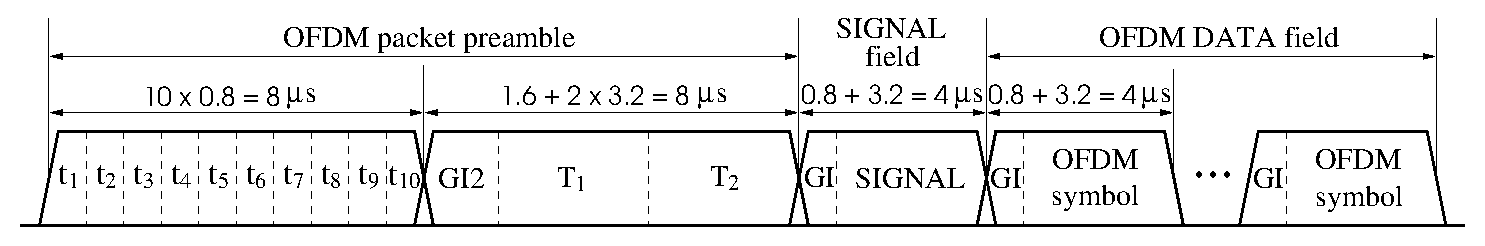
\includegraphics[height=0.8in]{fig/ofdmpacket_n.eps}
%\caption{Illustration of a packet defined by the IEEE 802.11a standard.} %
%\label{fig_sisopreamble}
%\end{figure*}

For the simulation of the time-dispersive fading channels for the
OFDM-based communication systems, the FIR (finite impulse response)
filter channel model~\cite{Chayat1997} can be used. While this model
is simple and effective for the detection/decoding performance
evaluation, it cannot be used as the foundation based 
squarely on which (i.e., to exploit the specific characteristics) to
devise signal processing algorithms for channel parameter
estimation. This issue was first alluded 
in~\cite{BeekEdforsSandell1995} but largely overlooked by many
researchers in the wireless communication community. This neglect is
evidenced by the fact that hundreds of publications in the topic of
channel estimation for the OFDM-based communication systems base the
algorithms squarely on the FIR model. While the results seem
impressive, the algorithms can hardly be used in real applications.
Even after this issue was made more clearly in a few recent
publications~\cite{LiuLi2003c,LiuLi2004,LiuLi2006}, many researcher
still extensively use the FIR model for channel estimation, as
demonstrated by very recent publications.

This paper explains in detail the reason why the FIR channel model
is only an approximate one for the OFDM-based 
communication systems, trying to
discourage the inappropriate usage of this model, which can lead to
fruitless efforts. This paper also presents a realistic channel
model for the OFDM-based communication systems, which can be used to
access the channel parameter estimation algorithms realistically.

Note that, as will be discussed later in this paper, the FIR channel
model can be a very appropriate model for single-carrier
communication schemes, such as CDMA.

The remainder of this paper is organized as follows. %
Section~\ref{sec2}
overviews the generation of OFDM data symbols.
Section~\ref{sec3}
presents equivalent discrete channel responses for the realistic
channels for the OFDM-based communication systems and discuss in detail the
limitation of the FIR channel model.
Section~\ref{sec4}
provides a realistic channel model which can be used for assessment
of channel estimation algorithms for the OFDM-based systems. %
Finally, we conclude in Section~\ref{sec5}.



\section{OFDM Data Model}
\label{siso_The_FIR_Channel_Model}
\label{sec2}

Before discussing the channel model, let us consider the generation
of the OFDM data symbols, as exemplified by those specified by the
IEEE 802.11a standard. Let %
\ben
\xbf_{k} = \left [ \ba{c} x_{k,1} \\
   x_{k,2} \\
   \vdots \\
   x_{k,N_S} \ea \right ], \quad
k = 1, 2, \dots, K, %
\label{equ_siso_symbols} %
\een %
be a vector of $N_S = 64$ symbols, where $x_{k,n_S}$, $n_S = 1, 2,
\dots, N_S$, is the symbol modulating the $n_S$th subcarrier and is
equal to 0 for the null subcarriers (there are 12 null subcarriers,
with one being at the center of the spectrum for dc bias removal and
the other 11 being at the two sides of the spectrum for bandwidth
protection), 1 or $-1$ for the pilot tones (there are 4 pilot
tones), or a member in a constellation $\Ccal$ for information-carrying
subcarriers (there are 48 information-carrying subcarriers). Here $K$ is
the number of OFDM data symbols in a packet and $\Ccal$ is a finite
constellation, such as BPSK, QPSK, 16-QAM, or 64-QAM. Let
$\Wbf_{N_S} \in {{\mathbb C}}^{N_S\times N_S}$ be the FFT matrix.
Then the $k$th OFDM data symbol $\sbf_k$ corresponding to $\xbf_{k}$
is obtained by taking
IFFT of $\xbf_{k}$. That is, %
\ben %
\sbf_k = \Wbf^H_{N_S} \xbf_{k} / N_S, %
\een %
where $(\cdot)^H$ denotes the conjugate transpose. To facilitate
eliminating inter-symbol interference (ISI) caused by the
time-dispersive channel at the receiver, $\sbf_{k}$ is preceded by a
cyclic prefix (CP) or guard interval (GI) $\sbf_{k,C}$ formed using
the last $N_C = 16$ elements of $\sbf_k$.

By stacking the packet preamble and the OFDM symbols (together with
their corresponding CPs) in the SIGNAL and OFDM DATA field, we
obtain the entire packet $\sbf\in {{\mathbb
C}}^{(5+K)(N_S+N_C)\times 1}$. (Here 5 is due to the fact that the
length of the packet preamble is the same as that 
of~4 OFDM data symbols and that
the length of the SIGNAL field is the same as~1 OFDM data symbol.) Passing
$\sbf$ through a pair of D/A converters at a rate of $f_S = 20$~MHz
(for both the real and imaginary parts of $\sbf$) and the
corresponding lower-pass filters, we obtain the (complex) baseband
analog waveform $s (t)$ which is shown in 
Figure~\ref{fig_siso_waveform}.

%\begin{figure}[t]
%\centering
%%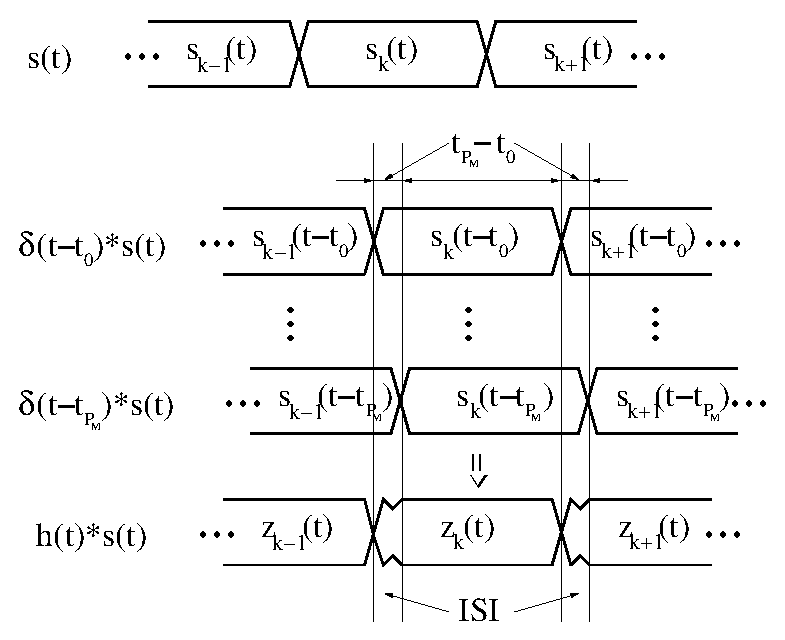
\includegraphics[height=2.5in]{fig/fig_datawaveform.eps}
%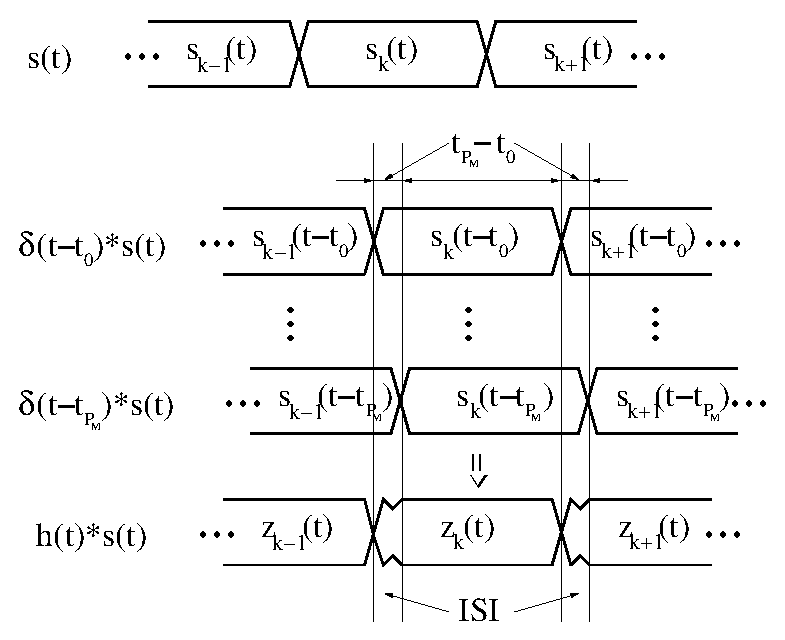
\includegraphics[height=3.2in]{fig/fig_datawaveform.eps}
%\caption{Illustrations of the analog waveforms for OFDM data symbols
%and the output of a multipath channel.} \label{fig_siso_waveform}
%\end{figure}



\section{Equivalent Discrete Channel Responses}
\label{sec3}

Let %
\ben %
h(t) = \sum_{p=0}^{P_M} \alpha_p \delta(t - t_p)
\label{equ_siso_ch_model1} %
\een %
denote the (baseband) time-domain {\em analog} channel impulse
response of a time-invariant multipath (aka, time-dispersive) fading
channel (called the {\em realistic channel} for short), where
$P_M$ is the number of multipaths, and
$\alpha_p$ and $t_p = \tau_p t_S$ ($\tau_0\le \tau_1 \le \dots \le
\tau_{P_M}$, $t_S = 1/f_S = 50$ ns) are the complex gain and time
delay of the $p$th path, respectively. Then the (baseband) input to
the receiver is %
\ben%
z(t) = h(t)*s(t), %
\een%
as shown in Figure~\ref{fig_siso_waveform}. To detect the data bits
contained in each OFDM data symbol, we need to sample $z(t)$ (with
sampling interval $t_S$) and process the sampled data in blocks of
length $N_S$. (Note that the samples are taken at the multiples of
$t_S$.)

Let %
\ben %
\hbf^{(\rm t)} = [h^{(\rm t)}_0 \fs h^{(\rm t)}_1 \fs \dots
   \fs h^{(\rm t)}_{N_S-1}]^T %
\label{equ_siso_equivalent_fir} %
\een %
be the corresponding time-domain {\em discrete} channel response,
referred to as the {\em equivalent} discrete channel response of
$h(t)$, for the sampled data blocks. Note that by {\em equivalence}
we mean that the discrete frequency-domain response 
of~(\ref{equ_siso_equivalent_fir}) is the same as the 
frequency-domain response 
of~(\ref{equ_siso_ch_model1}) on the (discrete) interested
subcarriers; i.e., if %
\ben %
{\hbf} = \Wbf_{N_S} \hbf^{(\rm t)} \defeq
[{h}_1 \fs {h}_2 \fs \dots \fs {h}_{N_S}]^T %
\een %
is the discrete frequency-domain channel response for the sampled
signals, then for an interested subcarrier $n_S$, we have: %
\ben %
{h}_{n_S} = \sum_p \left . \alpha_p e^{-j \tau_p t_S \omega }
   \right |_{\omega = \frac{2\pi [n_S-1]_{N_S}}{N_S t_S}},%
\label{equ_siso_fre_h_n_S} %
\een %
where %
\ben %
[n_S-1]_{N_S} = \left \{ \ba{ll}
   n_S - 1, & n_S \le N_S/2, \\
   n_S-1-N_S, & n_S > N_S/2. \ea \right .
\een %
Note that Equation~(\ref{equ_siso_fre_h_n_S}) implies that the
sampling starts from $t = 0$; to avoid ISI, we need to use correct
symbol timing. Note also that different symbol timing leads to different
phase expression in~(\ref{equ_siso_fre_h_n_S}).

We have two types of equivalent discrete channel responses depending
on the choices of the interested subcarriers, which are used to
transmit data. If we are interested in all of the $N_S = 64$
subcarriers, then we have the Type A equivalent
discrete channel response; 
the $l$th, $l = 0, 1, \dots, N_S-1$, element of
$\hbf^{(\rm t)}$ for the Type A equivalent
discrete channel response can be written as %
\ben %
h^{(\rm t)}_{l} =
\sum_p \alpha_p
      e^{j \frac{\pi (\tau_p-l)}{N_S}}
      \frac{\sin \left ( \pi (\tau_p-l) \right ) }
      {\sin \left ( \pi (\tau_p-l) / {N_S} \right ) }.
\label{equ_siso_ch_model1_1} %
\een %
On the other hand, if we are interested in only the $N_{SC} = 52$
non-zero subcarriers with the 12 null-subcarriers being set to zero,
then we have the Type B equivalent discrete channel response; 
the $l$th, $l = 0, 1, \dots, N_S-1$, 
element of $\hbf^{(\rm t)}$ for the Type B equivalent discrete 
channel response can be written as %
\ben h^{(\rm t)}_{l} =
\sum_p \alpha_p \left (
      \frac{\sin \left ( \pi (\tau_p-l) (N_{SC}+1) / N_S \right ) }
      {\sin \left ( \pi (\tau_p-l) / {N_S} \right ) } -1 \right ).
\label{equ_siso_ch_model1_N_SC} %
\een %
See Appendix~A.1 %\ref{app_siso_C} %
for the derivations of~(\ref{equ_siso_ch_model1_1}) 
and~(\ref{equ_siso_ch_model1_N_SC}).


Considering the above Type A and Type B equivalent discrete channel
responses, we have the following remarks pertaining to the FIR channel model
for the OFDM-based communication systems, which 
is assumed to have a time-domain length less
than $N_C$ so that the ISI problem can be eliminated.%
\begin{list}{}{
   \setlength{\leftmargin}{0.2in}
   \setlength{\itemindent}{-0.1in}
   }
\item[\bf Remark 1:] The time-domain lengths of both type of equivalent
discrete channel responses usually are $N_S$, as shown in 
Figure~\ref{fig_siso_equivalent_ch}. This is true even when we have only
one path where $t_0$ is not a multiple of $t_S$. The reason is that,
as shown in Figure~\ref{fig_siso_freq_ch}, the transition of
frequency-domain channel response from one period to another 
(around frequency indexes -32 and +32 in the figure) 
is not smooth due to
fact that $\tau_p$, ($p = 0, 1$ in this special case), 
is not an integer. As such, the FIR
channel model is only an {\em approximation} of the equivalent
discrete channel responses and hence an approximation of
a realistic channel
for the OFDM-based communication systems. Note that for an
FIR channel mode, the frequency-domain
channel response has a smooth transition from one period to another. 
Note also that the FIR channel
model can be very accurate for single-carrier communication schemes,
such as CDMA; this is detailed in Appendix~A.2.
%\ref{app_fir_for_cdma} .

\item[\bf Remark 2:] By restricting the delays in~(\ref{equ_siso_ch_model1})
to a few multiples of $t_S$, we have
\ben %
h_r (t) = \sum_{l_F=0}^{L_F -1} \alpha_{l_F} \delta(t -
l_F t_S ). %
\een %
In this case, the Type A equivalent discrete channel response 
of $h_r (t)$ will
have a length of $L_F$ (standing for length of FIR filter)
that is smaller than $N_S$, 
and $h_r (t)$ can be {\em exactly} expressed
by an FIR channel model. Note that this chance appears with a
possibility zero in real applications.

\item[\bf Remark 3:] Due to the above remarks, we stress that: (a)~the channel
parameter estimation methods for the OFDM-based communication systems cannot be
designed and assessed using the FIR channel model since channel
parameter estimation methods work well for the FIR channel may have
degraded performance for the realistic channels~\cite{LiuLi2004} and
(b)~the design of the packet preambles cannot be based on the time-domain
limited-duration property of the FIR channel model.
%\cite{LiuLi2007}.

\end{list}

The following notes can be helpful in explaining a few issues about
the equivalent discrete channel responses given above:%
\begin{list}{}{
   \setlength{\leftmargin}{0.2in}
   \setlength{\itemindent}{-0.1in}
   }
\item[\bf Note 1:] The length of the equivalent discrete channel responses, $N_S$,
is much longer than $N_C$, the length of CP. However, this will not
cause the ISI problem as long as $\tau_{P_M} - \tau_0 \le N_C-1$ and
we have the correct symbol timing. The reason is that the (sampled)
receiver output over the time-dispersive channel is {\em not}
obtained from the convolution of the equivalent discrete channel
response with $\sbf$; rather, it is obtained from sampling $z(t)$,
the convolution of $h(t)$ and $s (t)$, as shown in 
Figure~\ref{fig_siso_waveform}, with the portion contaminated by ISI
discarded by the correct symbol timing~\cite{LiuLi2004}.

\item[\bf Note 2:] In the case of perfect sampling clock synchronization,
i.e., the sampling clocks at the transmitter and receiver are
exactly the same, an equivalent discrete channel response, be it
Type A or Type B, is the same for all of the OFDM data symbols. In
the case of imperfect sampling clock synchronization, which is the
case for real applications, there will be sampling-shift that will
cause phase rotation for the equivalent discrete channel response.
This problem was addressed in detail in~\cite{LiuLi2004}.

\item[\bf Note 3:] If CFO simulation is needed, it should be
introduced at received signal, not the transmitted signal, as
detailed in Appendix A.3.

\end{list}



\section{A Realistic Channel Model}
\label{sec4}

For some simulation of the OFDM-based communication systems, the
equivalent discrete channel response $\hbf^{(\rm t)}$ can be {\em
approximated} by an exponentially decaying FIR channel response with
length $L_F$, denoted as
\ben %
h_e (t) = \sum_{l_F=0}^{L_F -1} h^{\rm (t)}_{l_F} \delta(t -
l_F t_S ), %
\label{equ_siso_ch_model2} %
\een %
where %
\ben %
h_{l_F}^{(\rm
t)} \sim \n \left ( 0, \left ( 1 - e^{-1/t_n} \right )
   e^{-l_F/t_n} \right ),
\label{equ_siso_fir_hl} %
\een %
with $ \left \{ h_{l_F}^{(\rm t)}
\right \}_{l_F = 0}^{L_F-1}$ being independent of each other, $t_n =
t_r / t_S$, $t_r$ being the root-mean-square (rms) delay spread of
the frequency-selective fading channel, $L_F = \lceil 10 t_n \rceil
+ 1$, and $\lceil x \rceil$ denoting the smallest integer not less
than $x$. This channel model is sometimes referred to as the
exponential channel model~\cite{Chayat1997}.

The exponential channel model is efficient for some numerical
simulations, such as the detection performance simulation; however,
as we have indicated earlier, this FIR channel model cannot be used
to assess the channel parameter estimation methods.

The realistic channel defined by~(\ref{equ_siso_ch_model1}) is fair
for the assessment of the channel parameter estimation methods, yet
the direct simulation of~(\ref{equ_siso_ch_model1}) is difficult due
to a potentially large $P_M$ and the distributions of $\alpha_p$.
Instead, we modify~(\ref{equ_siso_ch_model2}) slightly to better
characterize the realistic channels as follows:
\ben %
h_m (t) =
\sum_{l_F=0}^{L_F -1} h^{\rm (t)}_{l_F} \delta(t - l_F t_S -
t_{l_F}), %
\label{equ_siso_ch_model3} %
\een %
where $h^{\rm (t)}_{l_F}$
is as in~(\ref{equ_siso_fir_hl}) and $t_{l_F}$, $l_F = 0, 1, \dots,
L_F-1$, is uniformly distributed over $[0, t_S]$. We also assume
that $ \left \{ h_{l_F}^{(\rm t)} \right \}_{l_F = 0}^{L_F-1}$ and $
\left \{ t_{l_F} \right \}_{l_F = 0}^{L_F-1}$ are independent of
each other. This new channel model, referred to as the modified
exponential channel model, is more realistic than the one 
in~(\ref{equ_siso_ch_model2}) due to the time delays $ \left \{ t_{l_F}
\right \}_{l_F = 0}^{L_F-1}$ introduced 
in~(\ref{equ_siso_ch_model3}).

We have the following comments about the exponential channel model
of~(\ref{equ_siso_ch_model2}) and the modified exponential channel
model of (\ref{equ_siso_ch_model3}).
\begin{list}{}{
   \setlength{\leftmargin}{0.2in}
   \setlength{\itemindent}{-0.1in}
   }

\item[\bf Comment 1:]
The channel parameter estimation methods should be assessed by using
the modified exponential channel model~(\ref{equ_siso_ch_model3})
first. If they work well for this model, then a large amount of
simulations, especially those with detection, can be done using the
exponential channel model~(\ref{equ_siso_ch_model2}) due to the
points given in the following comment.

\item[\bf Comment 2:]
The exponential channel model is more efficient than the modified
exponential channel model for detection performance simulations. For
the exponential channel model, the sampled received data can be
easily obtained by convolving the channel $\hbf_{L_F}^{(\rm t)}$ and
the transmitted signal $\sbf$. For the modified exponential channel
model, on the other hand, the computation is much more complex, as
sketched below: (a)~take the FFT of the transmitted signal $\sbf$,
(b)~obtain the frequency-domain response of $h(t)$ similarly 
to~(\ref{equ_siso_fre_h_n_S}), and (c)~take the IFFT of the product of
the above two.

\item[\bf Comment 3:]
The channel model of~(\ref{equ_siso_ch_model3}) can be easily
extended to the multiple-input multiple-output (MIMO) case by using
the same $t_{l_F}$ but different $h^{\rm (t)}_{l_F}$ for each of the
MIMO channels.

\end{list}



\section{Conclusions}
\label{sec5}

As detailed in the paper, the FIR channel model cannot accurately
characterize the channels for the OFDM-based systems. Therefore
caution is needed when using this model for the OFDM-based systems.
It is especially not appropriate to design channel estimation
algorithms for the OFDM-based system squarely based on this model;
when this model is not appropriate, the modified exponential channel
model can be used.



\section*{\bf Appendixes}


\subsection*{A.1. Derivations of Equations
(\ref{equ_siso_ch_model1_1}) and (\ref{equ_siso_ch_model1_N_SC})}
\label{app_siso_C}

First, let us recall that the frequency-domain channel response
corresponding to the sampled signals is expressed as: %
\ben %
{h}_{n_S}
= \sum_p \alpha_p e^{-j \frac{2\pi \tau_p [n_S-1]_{N_S}}{N_S}},
   \quad n_S = 1, 2, \dots, N_S,
%\label{equ_siso_fre_h_n_S}
\een %
where %
\ben [n_S-1]_{N_S} = \left \{ \ba{ll}
   n_S - 1, & n_S \le N_S/2, \\
   n_S-1-N_S, & n_S > N_S/2. \ea \right .
\een

Second, let us derive Equation~(\ref{equ_siso_ch_model1_1}) with the
above expression. The $l$th, $l = 0, 1, \dots, N_S-1$, element of
the Type A equivalent discrete channel response of $h(t)$ can be
written as, due to the inverse DFT of ${h}_{n_S}$,
\begin{eqnarray}
h^{(\rm t)}_{l} & \bs = \bs &
   \sum_{n_S = 1}^{N_S}
   \left (\sum_p \alpha_p e^{-j \frac{2\pi \tau_p [n_S-1]_{N_S}}{N_S}}
      \right ) e^{j \frac{2 \pi l (n_S-1)}{N_S}}
\label{equ_siso_wlan_ch_model_key} \\
        & \bs = \bs &
   \sum_{n = -N_S/2}^{N_S/2-1}
   \left (\sum_p \alpha_p e^{-j \frac{2\pi \tau_p n}{N_S}}
      \right ) e^{j \frac{2 \pi l n}{N_S}} \nonumber \\
        & \bs = \bs &
   \sum_p \alpha_p \sum_{n = -N_S/2}^{N_S/2-1}
   e^{-j \frac{2\pi (\tau_p-l) n}{N_S}} \nonumber \\
        & \bs = \bs &
   \sum_p \alpha_p e^{j {\pi (\tau_p-l)}}
      \sum_{n = 0}^{N_S-1}
      e^{-j \frac{2\pi (\tau_p-l) n}{N_S}} \nonumber \\
        & \bs = \bs &
   \sum_p \alpha_p e^{j {\pi (\tau_p-l)}}
      \frac{1 - e^{-j 2\pi (\tau_p-l) } }
      {1- e^{-j \frac{2\pi (\tau_p-l) }{N_S}} } \nonumber \\
        & \bs = \bs &
   \sum_p \alpha_p
      e^{j \frac{\pi (\tau_p-l)}{N_S}}
      \frac{\sin \left ( \pi (\tau_p-l) \right ) }
      {\sin \left ( \pi (\tau_p-l) / {N_S} \right ) } .
\end{eqnarray}

Note that due to the failure of adequately addressing the
$[\cdot]_{N_S}$ problem in~(\ref{equ_siso_wlan_ch_model_key}), i.e.,
mistakenly using $n_S - 1$ instead of $[n_S - 1]_{N_S}$, which put
the discontinued points of the periodic frequency-domain response at
$\dots,-64, 0, 64, \dots$ rather than $\dots, -32, 32, \dots$ (cf.
Figure~\ref{fig_siso_freq_ch}), \cite{BeekEdforsSandell1995}
gives an inaccurate result as: %
\ben %
h^{(\rm t)}_{l} = \sum_p
\alpha_p e^{-j \pi (l + (N_S - 1) \tau_p )/{N_S}}
   \frac{\sin (\pi \tau_p)}{ \sin (\pi (\tau_p - l)/{N_S})}.
\label{equ_siso_ch_model1_wrong} %
\een

Third, let us derive Equation~(\ref{equ_siso_ch_model1_N_SC}). Using
the same approach as before, the $l$th element of the Type B
equivalent discrete channel response of $h(t)$ can be written as:
\begin{eqnarray}
h^{(\rm t)}_{l} & \bs = \bs &
   \sum_p \alpha_p \left ( \sum_{n = -N_{SC}/2}^{N_{SC}/2}
   e^{-j \frac{2\pi (\tau_p-l) n}{N_S}} -1 \right ) \nonumber \\
        & \bs = \bs &
   \sum_p \alpha_p \left ( e^{j \frac{\pi (\tau_p-l) N_{SC}}{N_S}}
      \sum_{n = 0}^{N_{SC}}
      e^{-j \frac{2\pi (\tau_p-l) n}{N_S}} -1 \right ) \nonumber \\
        & \bs = \bs &
   \sum_p \alpha_p \left ( e^{j \frac{\pi (\tau_p-l) N_{SC}}{N_S}} \,
      \frac{1 - e^{-j \frac{2\pi (\tau_p-l) (N_{SC}+1) }{N_S} } }
      {1- e^{-j \frac{2\pi (\tau_p-l) }{N_S}} } -1 \right ) \nonumber \\
        & \bs = \bs &
   \sum_p \alpha_p \left (
      \frac{\sin \left ( \pi (\tau_p-l) (N_{SC}+1) / N_S \right ) }
      {\sin \left ( \pi (\tau_p-l) / {N_S} \right ) } -1 \right ).
\end{eqnarray}



\subsection*{A.2. The FIR channel model for single-carrier
communication systems} %
\label{app_fir_for_cdma} %

Even though we have shown that the FIR channel model is only an
approximate one for the OFDM-based communication systems, this model
can be an accurate one for the single-carrier (SC) communication
systems, such as the CDMA systems. This can be understood from the
following two aspects.

First, the OFDM-based communication systems often aim at achieving
higher transmission data rate by using larger constellations, such
as 64-QAM, and thereby requiring higher signal-to-ratio (SNR)
compared to the SC systems. While a certain amount of approximation
is tolerable for the SC systems, it may cause serious problem for
the OFDM-based systems.

Second, which is more important, the SC systems often use the
limited-duration information-carrying pulses. For this kind of
pulses, an integrate-and-dump (IND) filter (can be a matched filter)
will have no output if there is no overlapping between the
integration time and the pulse duration; see, for example,
\cite{LiLiMiller2001} and the references therein. For instance, if
we use the rectangular pulse with duration $t_S$ and use the IND
filter which delivers its output every $t_S$ second, then the
non-zero outputs can be at most $\lceil \tau_{P_M} - \tau_0 +
1\rceil$ long for the channel given in~(\ref{equ_siso_ch_model1}),
which is a perfect FIR channel response. (Here $\lceil x \rceil$
stands for the smallest integer that is not smaller than $x$.)

The fact that the FIR channel model can be an accurate model for the
SC communication systems is perhaps the main reason that some
researchers use this model without scrutinizing in the OFDM-based
systems.


\subsection*{A.3. A note on the CFO effect simulation}
\label{app_siso_F}

The CFO is the difference between the oscillators at the transmitter
and receiver ends. It seems that this difference can be added at
either the transmitted signal, $s(t)$, or the received signal,
$z(t)$. (For notational convenience, We use the analog signals to
make our points.) This can be true for the case of estimated channel
parameters. Yet, for the case of perfect channel knowledge, special
attention should be paid for the simulation of CFO. If the CFO is
added on the received signal, everything is fine. If, on the other
hand, the CFO is added on the transmitted signal, a compensation
should be made to the channel response. This can be seen from the
following:
\begin{eqnarray}
& & \bs \bs \bs \bs \bs
   h(t) * \left ( s(t) e^{j 2\pi f_S \epsilon
t} \right ) \nonumber \\
      & \bs = \bs &
   \int s(t-\tau) e^{j 2\pi f_S \epsilon (t - \tau)} h(\tau) d \tau \nonumber \\
      & \bs = \bs &
   e^{j 2\pi f_S \epsilon t } \int s(t-\tau) h(\tau) e^{- j 2\pi f_S \epsilon \tau} d \tau \nonumber \\
      & \bs = \bs &
   e^{j 2\pi f_S \epsilon t } \left [ z(t) *
      \left ( h(t) e^{- j 2\pi f_S \epsilon t} \right ) \right ],
\end{eqnarray}
where $h(t) e^{- j 2\pi f_S \epsilon t}$ is the actual channel
response for this case.


\newpage

%\spacingset{1.025}
\bibliographystyle{ieeetr}
\bibliography{../../commonFiles/all}
%\bibliography{C:/Users/jhl/OneDrive/docs/dcgn/all}


\newpage

\begin{figure*}[t]
\centering
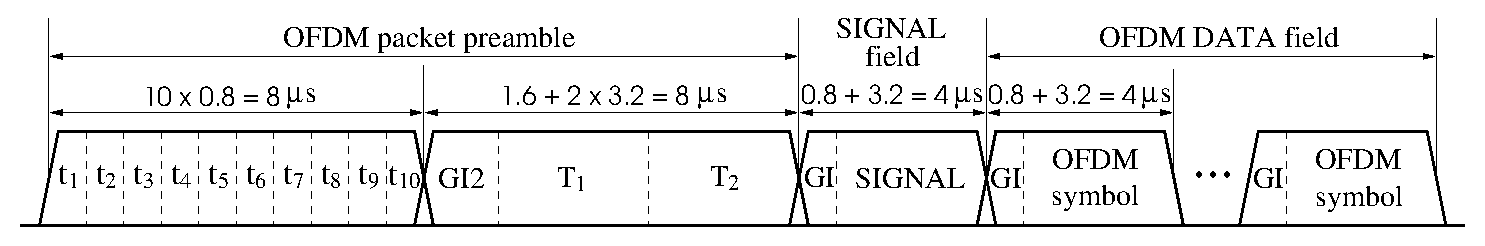
\includegraphics[height=1.0in]{fig/ofdmpacket_n.eps}
\caption{Illustration of a packet defined by the IEEE 802.11a standard.} %
\label{fig_sisopreamble}
\end{figure*}

\begin{figure}[t]
\centering
%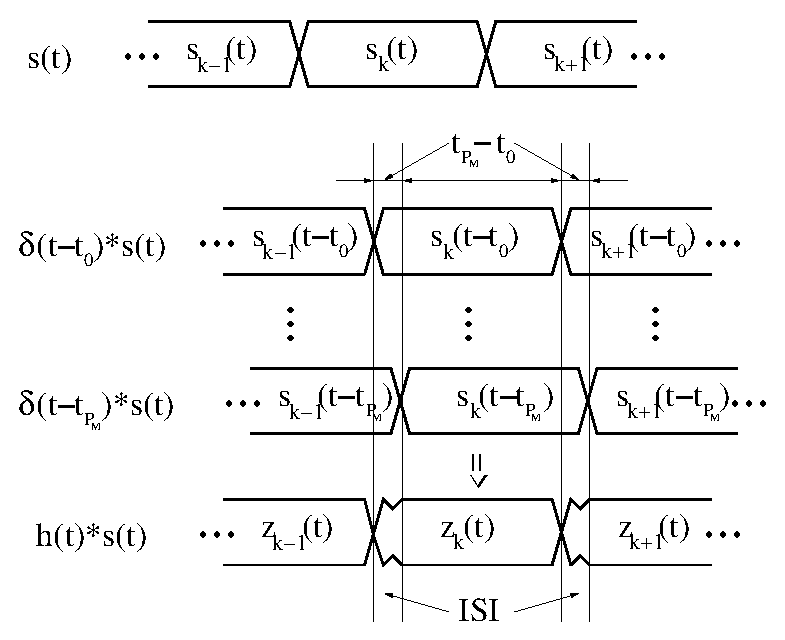
\includegraphics[height=2.5in]{fig/fig_datawaveform.eps}
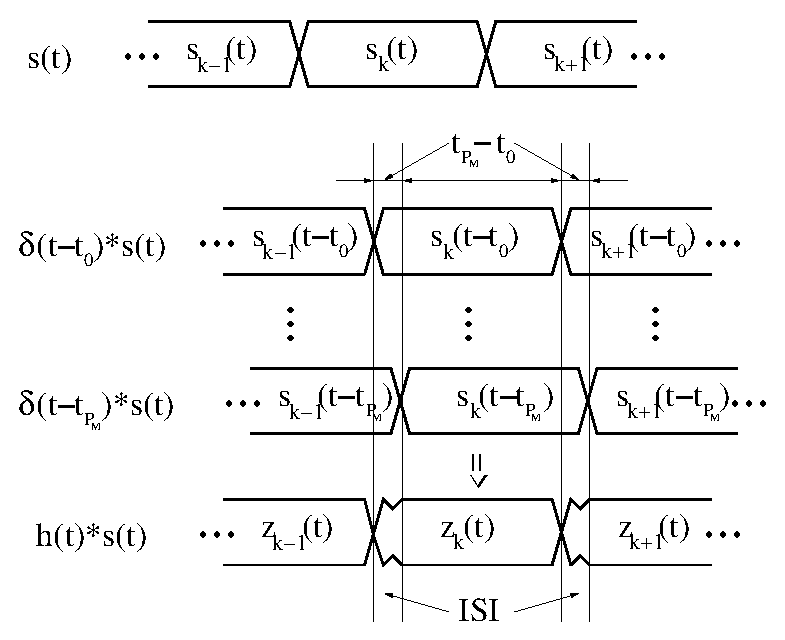
\includegraphics[height=3.2in]{fig/fig_datawaveform.eps}
\caption{Illustrations of the analog waveforms for OFDM data symbols
and the output of a multipath channel.} \label{fig_siso_waveform}
\end{figure}

\begin{figure}[t]
\centering
\begin{tabular}{c}
%\hspace{-0.15in}
%\includegraphics[height=2.5in]{fig/fig_equivalent_ch1.eps} \\
\includegraphics[height=3.2in]{fig/fig_equivalent_ch1.eps} \\
(a) \\
%\hspace{-0.2in}
%\includegraphics[height=2.5in]{fig/fig_equivalent_ch2.eps} \\
\includegraphics[height=3.2in]{fig/fig_equivalent_ch2.eps} \\
(b)
\end{tabular}
\caption{Illustration of the amplitude of two types of equivalent
discrete channel response for a multipath channel described by $h(t)
= \delta(t - 2.5 t_S) - j 0.5 \delta(t - 4.8 t_S)$: (a) Type A; (b)
Type B.} \label{fig_siso_equivalent_ch}
\end{figure}

\begin{figure}[t]
\centering
\begin{tabular}{c}
%\psfig{figure=/home/sal/jhliu/work/ofdm/papers/sisotiming/fig_equivalent_ch3.eps,height=2.5in}
%\includegraphics[height=2.5in]{fig/fig_equivalent_ch3.eps}
\includegraphics[height=3.2in]{fig/fig_equivalent_ch3.eps}
\end{tabular}
\caption{Illustration of the discontinuities in the amplitude of the
frequency-domain channel response for a multipath channel described
by $h(t) = \delta(t - 2.5 t_S) - j 0.5 \delta(t - 4.8 t_S)$.}
\label{fig_siso_freq_ch}
\end{figure}


\end{document}
